\documentclass{beamer}
% Change theme
\usetheme{Antibes}
\usecolortheme{beaver}
% Change font
\usepackage[T1]{fontenc}
\usepackage[]{kpfonts}
% Use cleveref package
\usepackage[capitalise]{cleveref}
% Use tikz
\usepackage[]{tikz}
\usetikzlibrary{backgrounds}
% Use bbm for blackboard things
\usepackage[]{bbm}
% Bibliography
\usepackage[
backend=biber,
style=authoryear-comp,
sorting=ynt,
url=false,
isbn=false,
doi=false
]{biblatex}
\AtEveryBibitem{%
  \clearfield{note}%
  \clearfield{eprinttype}%
  \clearfield{eprint}%
}
\addbibresource{Library.bib}
% Pictures path
\graphicspath{{./Pictures/}}
% Remove controls
\beamertemplatenavigationsymbolsempty 

% Title page information
\title{Approximation of Generalised Functions for Numerical Solutions of SDEs}
\author{Luis-Mario Chaparro-Jáquez}
\institute{University of Leeds\\School of Mathematics}
\date{December 8th 2021}
\logo{
\includegraphics[width=25mm]{logo_leeds}}
% Table of contents at the beginning of each section
\AtBeginSection[]
{
  \begin{frame}{Table of Contents}
    \tableofcontents[currentsection]
  \end{frame}
}

\begin{document}
\frame{\titlepage}
\frame{\tableofcontents}
\section{SDEs with distributional coefficients}
\begin{frame}{SDEs with distributional coefficients}
        Consider the SDE% as in
        %\cite{de_angelis_numerical_2020}
        \begin{equation*}
                \label{eq:distributional_sde}
                \begin{cases}
                        dX_t = b(t, X_t) dt + dW_t
                        &
                        \\
                        X_0 = x_0, \quad t \in [0,T],
                \end{cases}
        \end{equation*}
        where
        $(W_t)_{t \geq 0}$
        is a Brownian motion, and
        $b$
        belongs to a Sobolev space
        $H^{-s}_p(\mathbb{R})$
        of negative and non-integer order, in particular
        $b$
is a distribution.
\end{frame}

\section{What is an SDE?}
\begin{frame}{What is an SDE?}
        Let
        $ (\Omega, \mathcal{F}, \mathbb{F}, W_{t}) $
        be a filtered probability space, a Stochastic Differential Equation (SDE) is a relation
        \begin{equation*}
                \label{eq:sde}
                X_{t} = x + \int_{0}^{t} b(X_{t}, t) dt + \int_{0}^{t} \sigma(X_{t}, t) dW_{t}.
        \end{equation*}
        \pause
        {\color{red}
        It is also denoted by
        \begin{equation*}
                \begin{cases}
                        dX_{t} = X_{0} + b(X_{t}, t) dt + \sigma(X_{t}, t) dW_{t}
                        \\
                        X_0 = x
                \end{cases}.
        \end{equation*}
        }

\end{frame}

\subsection{Solutions of SDEs}
\begin{frame}{Solutions of SDEs}
        \begin{definition}[Strong solution of an SDE]
                If for a Brownian motion
                $ (W_{t})_{t \ge 0} $
                there exist a process
                $ (X_{t})_{t \ge 0} $
                satisfying
                \eqref{eq:sde}
                $ \mathbb{P} $-almost surely
                we say that the SDE has a strong solution.
        \end{definition}


\end{frame}

\begin{frame}{Existence and uniqueness}
        \begin{theorem}[{{\cite[]{karatzas_brownian_1991}}}]
                \label{th:sde_soln}
                Suppose that there exists a constant
                $ K \ge 0 $
                such that for all
                $ x, y \in \mathbb{R} $
                and
                $ t \in [0,T] $,
                \begin{equation*}
                        | b(t,x) - b(t,y) | + | \sigma(t,x) - \sigma(t,y) | \le K | x - y|
                \end{equation*}
                and
                \begin{equation*}
                        | b(t,x) | + | \sigma(t,x) | \le K (1 - | x |).
                \end{equation*}
                Then there exist a continuous
                $ \mathbb{F} $-adapted
                process
                $ (X_{t})_{t \ge 0} $
                which is a strong solution to
                \label{eq:sde},
                which is unique up to indistinguishability.
        \end{theorem}
\end{frame}

\subsection{Numerical schemes for SDEs}
\begin{frame}{Numerical schemes for SDEs}
        \begin{definition}[Euler scheme]
                Let
                $ (t_{n})_{n=0}^{N} $
                be a discretisation of the interval
                $ [0,T] $.
                Then an Euler approximation for the solution of the SDE
                \label{eq:sde}
                at time
                $ t_{n+1} $
                is given by
                \begin{equation*}
                        Y_{n+1} = b(t, Y_{n}) \Delta t_{n} + \sigma(t, Y_{n}) \Delta W_{n}
                \end{equation*}
        \end{definition}
\end{frame}

\begin{frame}{Strong convergence rate of Euler scheme}
        \begin{theorem}[{{\cite[]{kloeden_numerical_1999}}}]
                Suppose conditions from
                \cref{th:sde_soln}
                for coefficients
                $ b $
                and
                $ \sigma $ 
                hold.
                Additionally assume that for any
                $ 0 \le s < t \le T $,
                \begin{equation*}
                        \label{eq:ext_lin_g}
                        | b(s, x) - b(t, x) | + | \sigma(s, x) - \sigma(t, x) |
                        \leq
                        K (1 + |x|) \sqrt{| t - s |},
                \end{equation*}
                holds.
                Then there exist a constant
                $ M < \infty $
                such that
                \begin{equation*}
                        \mathbb{E} | X_T - Y_N | \leq M \left( \max_{n} \Delta t_n \right)^{\frac{1}{2}},
                \end{equation*}
                where
                $ X $
                is the real solution
                $ Y $
                the approximated solution and
                $ (t_{n})_{n=0}^{N} $
                a time grid.
        \end{theorem}

\end{frame}


\section{What is a distribution/generalised function?}
\begin{frame}{What is a distribution?}
        \begin{definition}[Distribution]
                Let 
                $ f \in \mathcal{D}(\mathbb{R}) := C^{\infty}_{c}(\mathbb{R}) $
                then a distribution or generalised function is a linear mapping 
                $ \phi \mapsto (f, \phi) $
                from
                $ \mathcal{D}(\mathbb{R}) $
                to
                $ \mathbb{R} $
                such that if
                $ \phi_{n} \to \phi $
                in
                $ \mathcal{D}(\mathbb{R}) $
                then
                $ (f, \phi_{n}) \to (f, \phi) $
                in
                $ \mathbb{R} $
                We denote the space of distributions as
                $ \mathcal{D}'(\mathbb{R}) $.
        \end{definition}
        \pause
        In particular we use a space of distributions
        \begin{equation*}
                I^{-s}L^p(\mathbb{R}) =: {\color{red} H^{s}_{p}(\mathbb{R})} \subset \mathcal{S}'(\mathbb{R}) \subset \mathcal{D}'(\mathbb{R}),
        \end{equation*}
        for
        $ s < 0 $
        and
        \begin{equation*}
                I^{s}: f \mapsto \mathcal{F}^{-1} \left[ \left( 1 + |\xi|^{2} \right)^{\frac{s}{2}} \mathcal{F} \left[ f \right] \right],
        \end{equation*}
        and
        $ f \in \mathcal{S}'(\mathbb{R}) $.
\end{frame}

\section{Approximation with Haar functions}

\begin{frame}{A picture of Haar and Faber functions}
        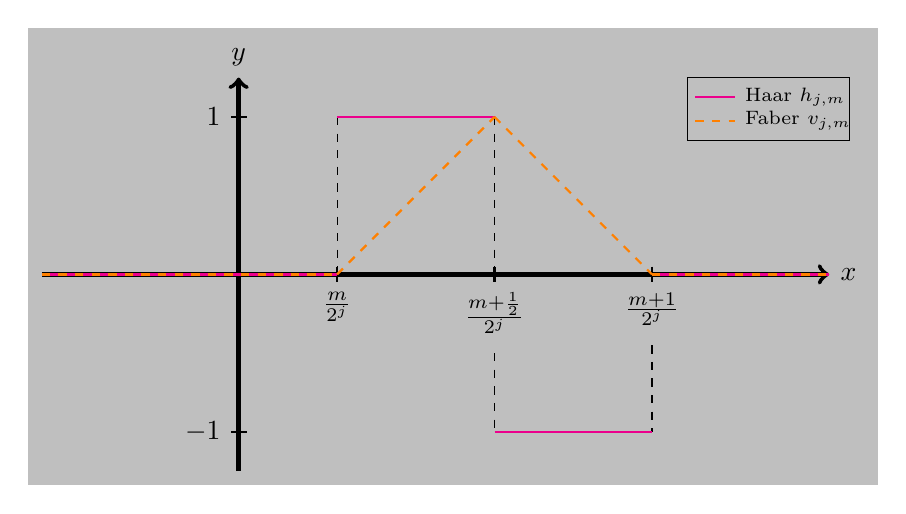
\begin{tikzpicture}[background rectangle/.style={fill=lightgray}, show background rectangle]
              % X and Y axis
              \draw[->, ultra thick] (-5,2.5)--(5,2.5) node[right]{$x$};
              \draw[->, ultra thick] (-2.5,0)--(-2.5,5) node[above]{$y$};
              % Help lines
              \draw[thin, dashed] (-1.25, 4.5)--(-1.25,2.5);
              \draw[thin, dashed] (0.75, 4.5)--(0.75,2.5);
              \draw[thin, dashed] (0.75, 1.5)--(0.75,0.5);
              \draw[thin, dashed] (2.75, 1.6)--(2.75,0.5);
              % Notable points for the graph
              \draw[thick] (-2.4,4.5)--(-2.6,4.5) node[left]{$1$};
              \draw[thick] (-2.4,0.5)--(-2.6,0.5) node[left]{$-1$};
              \draw[thick] (-1.25,2.6)--(-1.25,2.4) node[below]{$\frac{m}{2^{j}}$};
              \draw[thick] (0.75,2.6)--(0.75,2.4) node[below]{$\frac{m+\frac{1}{2}}{2^{j}}$};
              \draw[thick] (2.75,2.6)--(2.75,2.4) node[below]{$\frac{m+1}{2^{j}}$};
              % Haar function
              \draw[magenta, thick] (-5,2.5)--(-1.25,2.5);
              \draw[magenta, thick] (-1.25,4.5)--(0.75,4.5);
              \draw[magenta, thick] (0.75,0.5)--(2.75,0.5);
              \draw[magenta, thick] (2.75,2.5)--(5,2.5);
              % Faber function
              \draw[orange, thick] (-5,2.5)--(-1.25,2.5)[dashed];
              \draw[orange, thick] (-1.25,2.5)--(0.75,4.5)[dashed];
              \draw[orange, thick] (0.75,4.5)--(2.75,2.5)[dashed];
              \draw[orange, thick] (2.75,2.5)--(5,2.5)[dashed];
              % Legend
              \draw[very thin] (3.2,5) rectangle (5.25,4.2);
              \draw[magenta, thick] (3.3,4.75)--(3.8,4.75) node[color=black, right]{\scriptsize Haar $h_{j,m}$};
              \draw[orange, thick] (3.3,4.45)--(3.8,4.45)[dashed] node[color=black, right]{\scriptsize Faber $v_{j,m}$};

      \end{tikzpicture}  
\end{frame}

\begin{frame}{Approximation with Haar functions}
        \begin{theorem}[{{\cite[]{triebel_bases_2010}}}]
                {\footnotesize
                Let
                $ I = (0,1) $,
                $ 0 \le p < \infty $,
                $ - \frac{1}{2} < s < \frac{1}{p} $,
                and
                $ f \in \mathcal{D}'(I) $.
                Then
                $f \in H^{s}_{p}(I)$
                if and only if
                \begin{equation*}
                        f = \sum_{j=0}^{\infty} \sum_{m=0}^{2^j-1} \mu_{j,m} 2^{-j\left( s - \frac{1}{r} \right)} h_{j,m}.
                \end{equation*}
                The representation is unique with the coefficients given by
                \begin{equation*}
                        \mu_0 := \int_0^1 f(x) h_0(x) dx
                        \quad \text{and} \quad
                        \mu_{j,m} := 2^{j\left( s - \frac{1}{p} + 1 \right)} \int_{0}^1 f(x) h_{j,m}(x) dx
                \end{equation*}
                for
                $j\in\mathbb{N}$
                and
                $m=0,...,2^j-1$,
                {\color{red}where the integral above is in the sense of dual pairing}.
                }
        \end{theorem}
\end{frame}

\subsection{Faber functions}
\begin{frame}{Faber functions}
        \begin{theorem}[{{\cite[]{triebel_bases_2010}}}]
                {\footnotesize
                Let
                $ I = (0,1) $,
                and
                $f \in H^{s}_{p}(I)$
                $ 2 \le p < \infty $,
                $ \frac{1}{2} < s < 1+\frac{1}{p} $,
                then
                \begin{equation*}
                        g = \hat{\mu}_0 v_0 + \hat{\mu}_1 v_1 + \sum_{j=0}^{+\infty} \sum_{m=0}^{2^{j} - 1} \hat{\mu}_{j,m} v_{j,m}
                \end{equation*}
                The representation is unique with the coefficients given by
                \begin{equation*}
                        \begin{cases}
                                \hat{\mu}_{j,m} &= -\frac{1}{2} (\Delta^{2}_{2^{-j-1}} g)(2^{-j} m)
                                \\
                                \hat{\mu}_0 &= g(0)
                                \\
                                \hat{\mu}_1 &= g(1),
                        \end{cases}
                \end{equation*}
                $(\Delta^{2}_{h} g) (x) := g(x + 2h) - 2g(x + h) + g(x)$.
                }
        \end{theorem}

\end{frame}

\begin{frame}{How to deal with the dual pairing}
        Since a Haar function
        $ h_{j,m} $
        is the same as the derivative of a Faber function
        $ v_{j,m} $.
        Thanks to the series representations stated before we can think of a function
        $ f \in H^{s-1}_{p} $
        as
        $ f = \frac{dg}{dx} $
        where
       $ g \in H^{s}_{p} $
        for
        $ 2 \le p < \infty $
        and
        $ \frac{1}{2} < s < 1 + \frac{1}{p} $.
\end{frame}

\begin{frame}{How to deal with the dual pairing}
        \begin{theorem}[{{\cite[]{triebel_bases_2010}}}]
                Let
                $g \in H^{s}_{p}(I)$,
                then
                $g' \in H^{s-1}_{p}(I)$
                with
                $2 \leq p < \infty$,
                $\frac{1}{2} < s < 1 + \frac{1}{p}$
                which can be written as
                \begin{equation*}
                        g' = (\hat{\mu}_1 - \hat{\mu}_0)h_0 + \sum_{j=0}^{+\infty} \sum_{m=0}^{2^{j} - 1} 2^{j+1} \hat{\mu}_{j,m} h_{j,m},
                \end{equation*}
                where
                \begin{equation*}
                        \mu_{0} = \hat{\mu}_1 - \hat{\mu}_0 \qquad and \qquad \mu_{j,m} = 2^{j+1} \hat{\mu}_{j,m}.
                \end{equation*}
        \end{theorem}
\end{frame}

\begin{frame}{Definition of our coefficient}
        \small
        We select our drift coefficient (which we consider time homogeneous) as the derivative with respect to
        $ x $
        of a single path of fractional Brownian motion
        $ B^{H}(x) \in H^{s}_{p} $,
        i.e:
        \begin{equation*}
                b = \frac{d}{dx}B^{H}(x) = \mu_{0} h_{0}(x) + \sum_{j=0}^{\infty} \sum_{m=0}^{2^{j} - 1} \mu_{j,m} h_{j,m}(x),
        \end{equation*}
        \pause
        and then our approximation to the coefficient would be
        \begin{equation*}
                \color{red}
                b^{N} = \mu_{0} h_{0}(x) + \sum_{j=0}^{N} \sum_{m=0}^{2^{j} - 1} \mu_{j,m} h_{j,m}(x).
        \end{equation*}
        \pause
        where
        \begin{equation*}
        \begin{cases}
                \mu_{0} &= B^{H}(1) - B^{H}(0)
                \\
                \mu_{j,m} &= -2^j \left( B^H \left( \frac{m+1}{2^j} \right) -2B^H \left( \frac{m + \frac{1}{2}}{2^j} \right) + B^H \left( \frac{m}{2^j} \right) \right).
        \end{cases}
        \end{equation*}
\end{frame}

\subsection{The heat semigroup}
\begin{frame}{The heat semigroup}
        \begin{definition}
                The heat kernel is a function
                $ \phi(t,x): [0,T] \times \mathbb{R} \to \mathbb{R} $
                defined as
                \begin{equation*}
                        \phi(t,x) := \frac{1}{\sqrt{2 \pi t} } \exp \left( - \frac{x^{2}}{2t}\right) .
                \end{equation*}
        \end{definition}
        To make the coefficient
        $ b^{N} $
        smooth we apply the heat kernel via convolution, denoted as
        \begin{equation*}
                P_{\eta_{N}} b^{N} (x) = (\phi * b^{N})(x) = \int_{-\infty}^{\infty} \phi(t, x - y) b^{N}(y) dy.
        \end{equation*}
        This is called {\color{red}heat semigroup}.
\end{frame}

\begin{frame}{The heat semigroup}
        And as
        $ b^{N} $
        is a sum of Haar functions, the heat semigroup computed over each elemen of that sum will be
        \begin{equation*}
                \begin{split}
                        [P_{\eta_{N}} h_{j,m}](x)
                        &=
                        \left[P_{\eta_{N}} \mathbbm{1}_{\left[\frac{m}{2^j}, \frac{m + 1/2}{2^j}\right)}\right](x)
                        - \left[P_{\eta_{N}} \mathbbm{1}_{\left[\frac{m + 1/2}{2^j}, \frac{m + 1}{2^j}\right)}\right](x)
                        \\
                        &=
                        \exp(-\eta_{N})
                        \left(
                        - \Phi \left( \frac{x - \frac{m + 1}{2^{j}}}{\sqrt{\eta_{N}}} \right)
                        + 2 \Phi \left( \frac{x - \frac{m + 1/2}{2^{j}}}{\sqrt{\eta_{N}}} \right)
                        - \Phi \left( \frac{x - \frac{m}{2^{j}}}{\sqrt{\eta_{N}}} \right)
                        \right).
                \end{split}
        \end{equation*}
\end{frame}

\section{A modified Euler scheme}
\begin{frame}{A modified Euler scheme}
        Given that now we have a ``nice'' approximation of the distributional coefficient we have the SDE
        \begin{equation*}
				\begin{cases}
						dX^N_t
						= P_{\eta_{N}} b^N(X^N_t) dt
						+ dW_t,
						\quad
						t \in [0, T]
						\\
						X^N_0 = x_0,
				\end{cases}
		\end{equation*}
		and the {\color{red}``Euler scheme''} will be
		\begin{equation*}
				Y^{N}_{n+1} = Y^{N}_{n} + P_{\eta_{N}} b^{N}(Y^{N}_{n}) \Delta t_{n} + \Delta W_{n}.
		\end{equation*}
\end{frame}

\subsection{Order of convergence}
\begin{frame}{Order of convergence}
		\begin{itemize}
		\item Combining the result that links the previous SDE with the original, and the result for the Euler scheme with the previous equation we will have that the ``Euler scheme'' to the real solution we will have a convergence rate of
		\begin{equation*}
				\frac{1}{2}\left( \frac{3}{4} - \beta_0 \left( \gamma_0 - \frac{1}{2} \right) \right)^{-1} \left( \frac{1}{2} - \beta_0 \right) \left( \gamma_0 - \frac{1}{2} \right) - \epsilon
		\end{equation*}
		for
		$ b \in H^{-\beta_0}_{q_0, \tilde{q}_0} $
		and
		$ \gamma_0  = 1 - \beta_0 - 1/q_0$
		where
		$\beta_0 \in (0,1/4)$,
		$q_0 \in (4, 1/\beta_0)$
		and
		$\tilde{q}_0 := (1 - \beta_0)^{-1}$
		is fixed.

		\pause
		\item As an example, if
		$\beta_0 = 0.05$,
		and
		$q_0 = 1/\beta_0$
		we have a convergence order of approximately {\color{red}0.12}
		(\cite[]{de_angelis_numerical_2020}).
		\end{itemize}
\end{frame}

\section{Implementation}
\begin{frame}{Implementation}
		\begin{figure}
				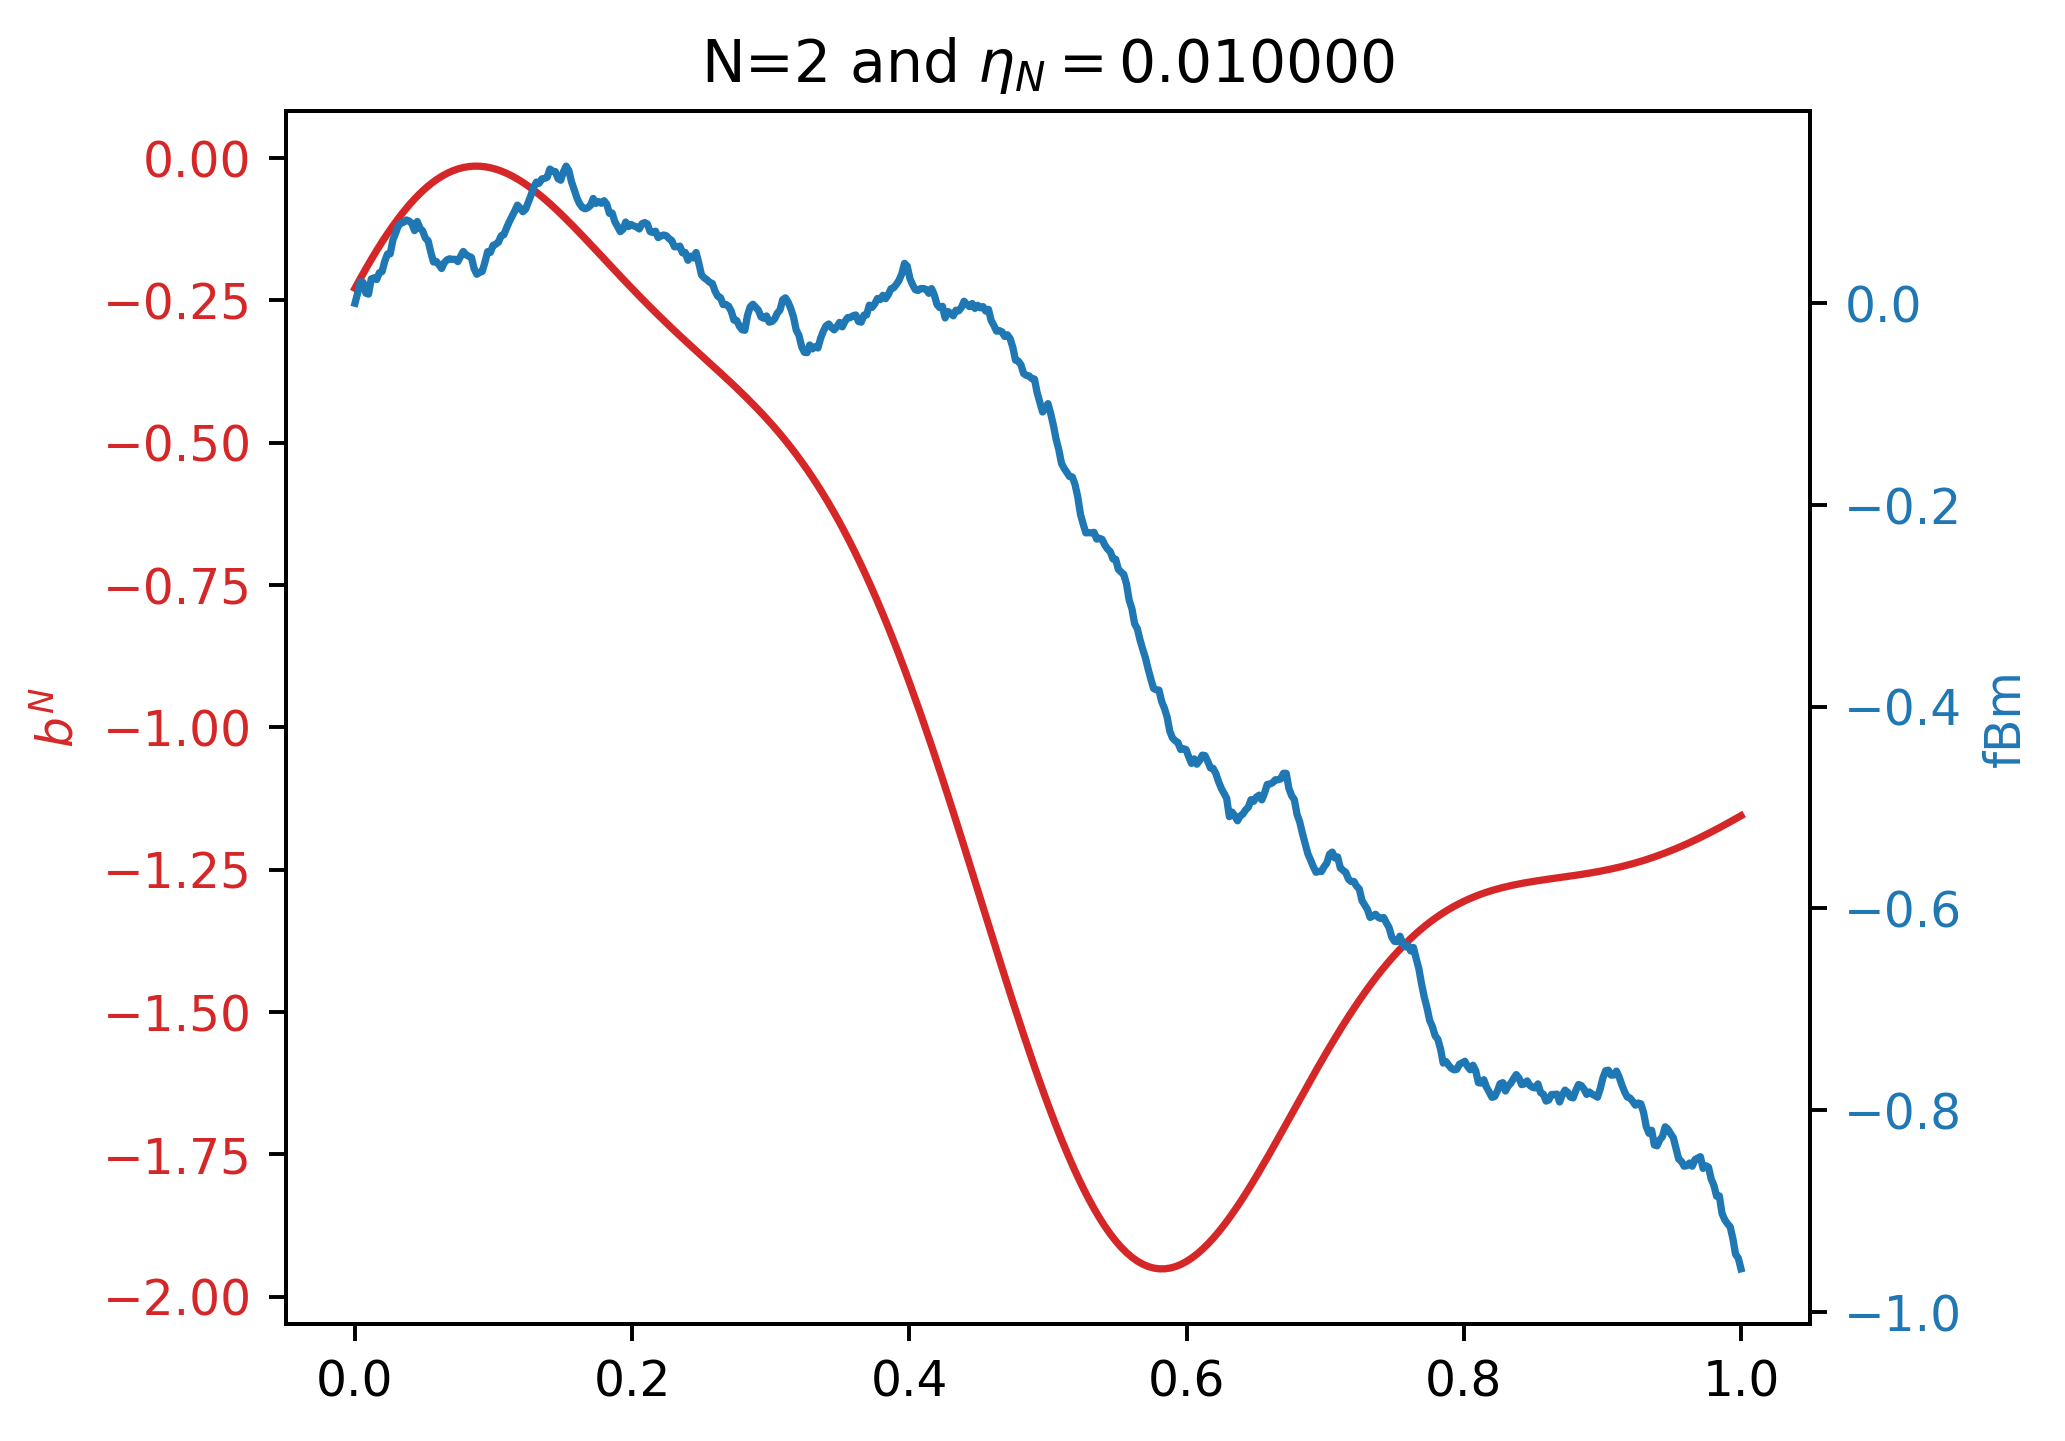
\includegraphics[width=0.49\textwidth]{bn_n2_eta01}
				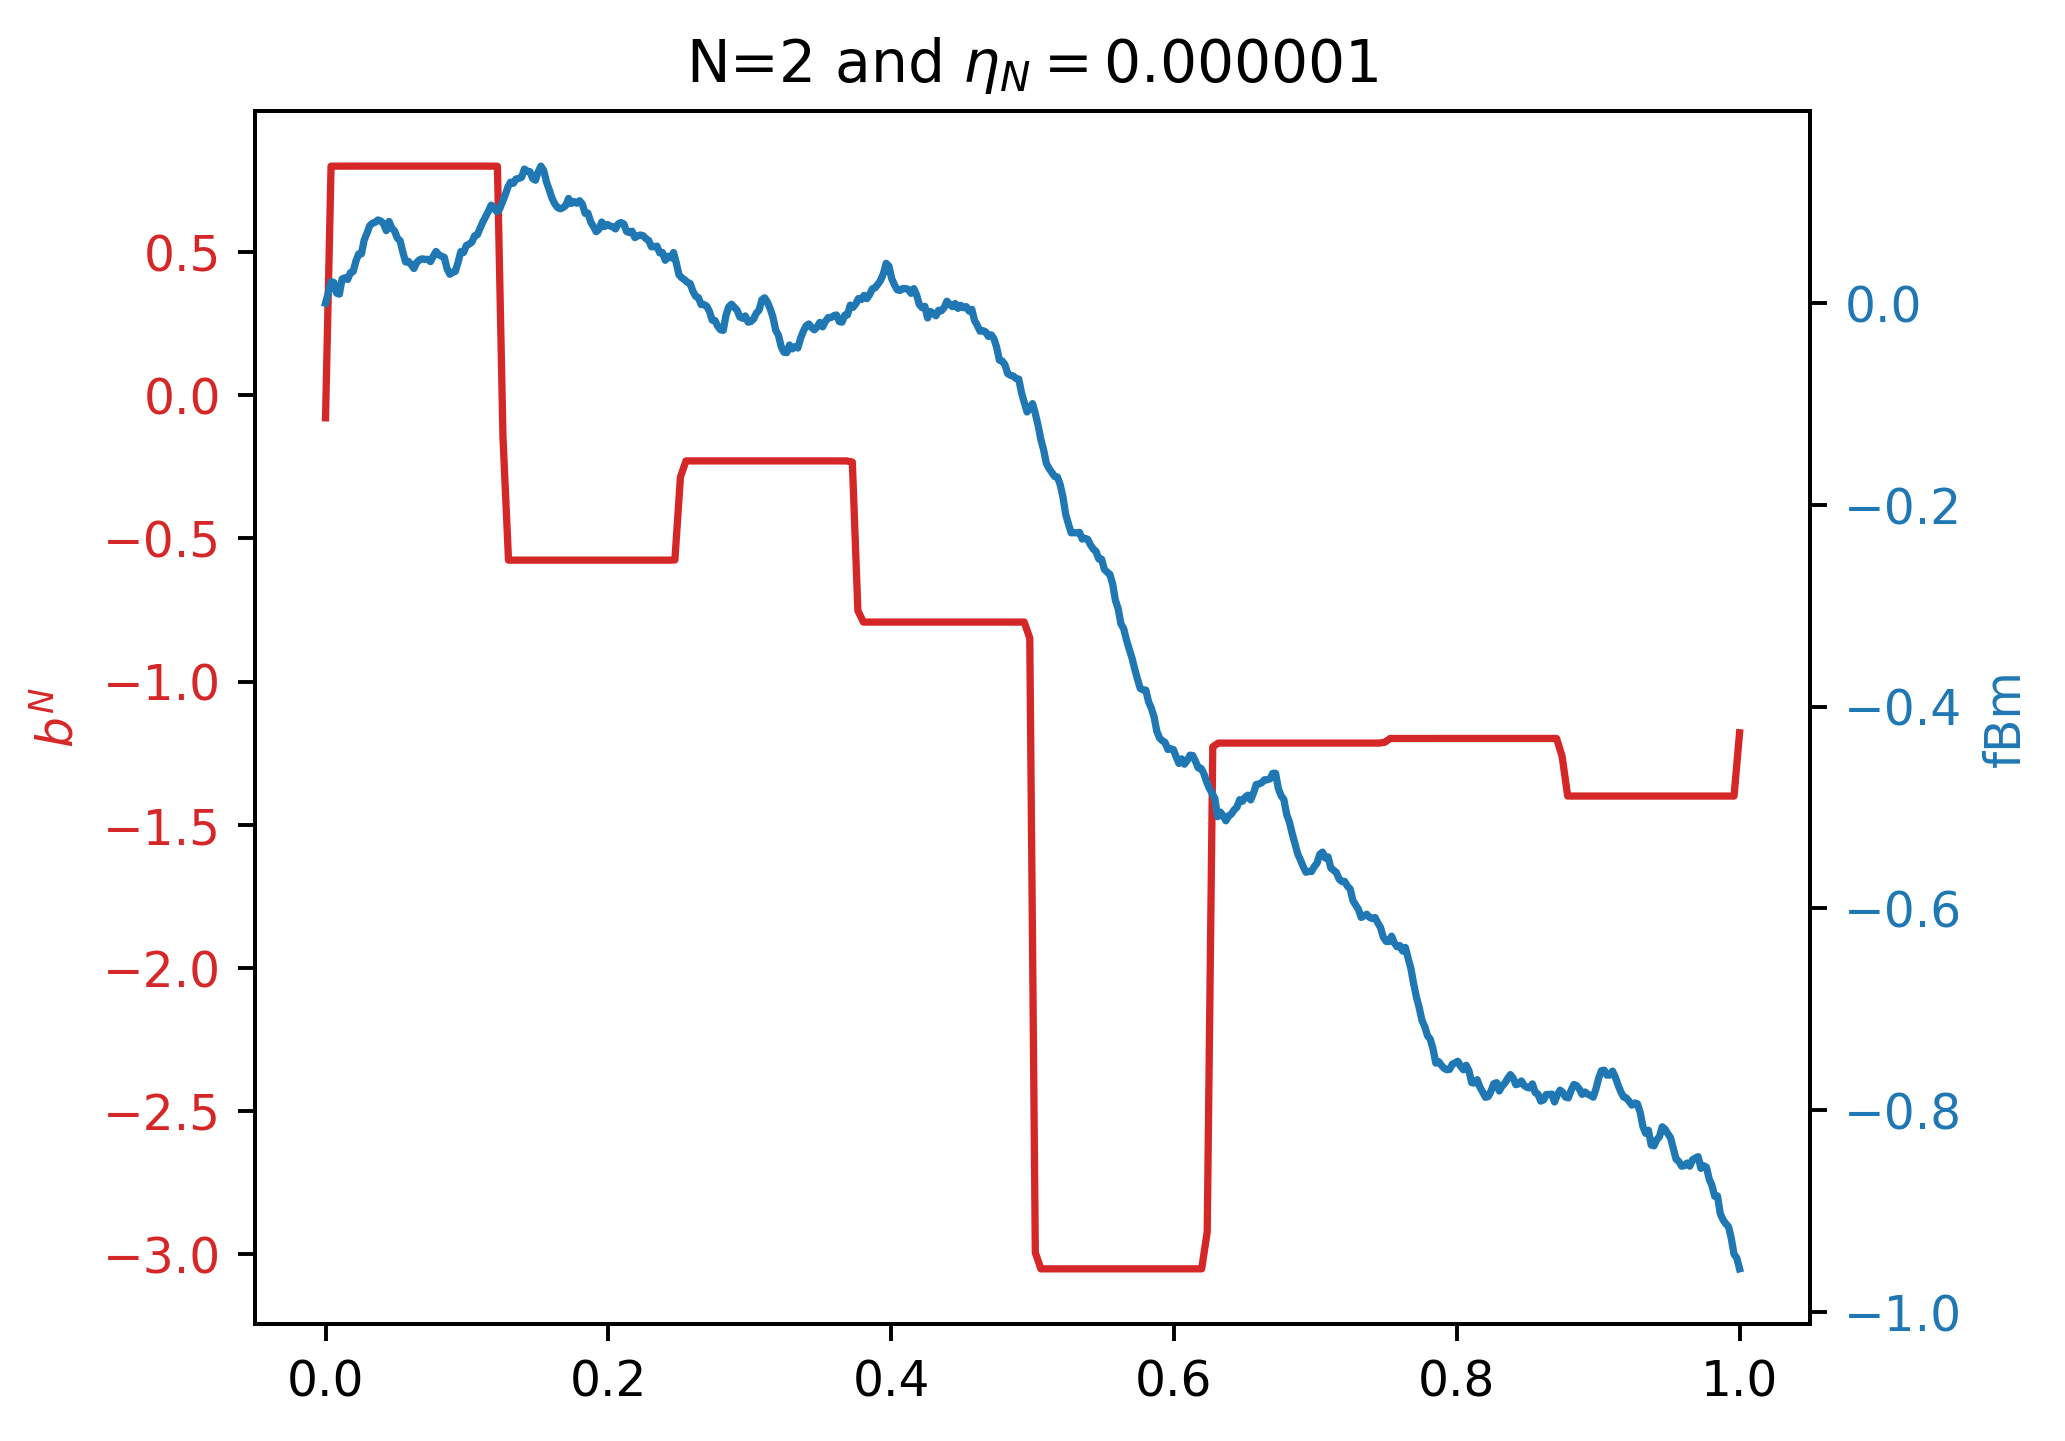
\includegraphics[width=0.49\textwidth]{bn_n2_eta501}
				\caption{Coefficient $P_{\eta_{N}}b^{N}$ for $N=2$ and $\eta=10^{-2}, 10^{-6}$.}
		\end{figure}
\end{frame}

\begin{frame}{Implementation}
		\begin{figure}
				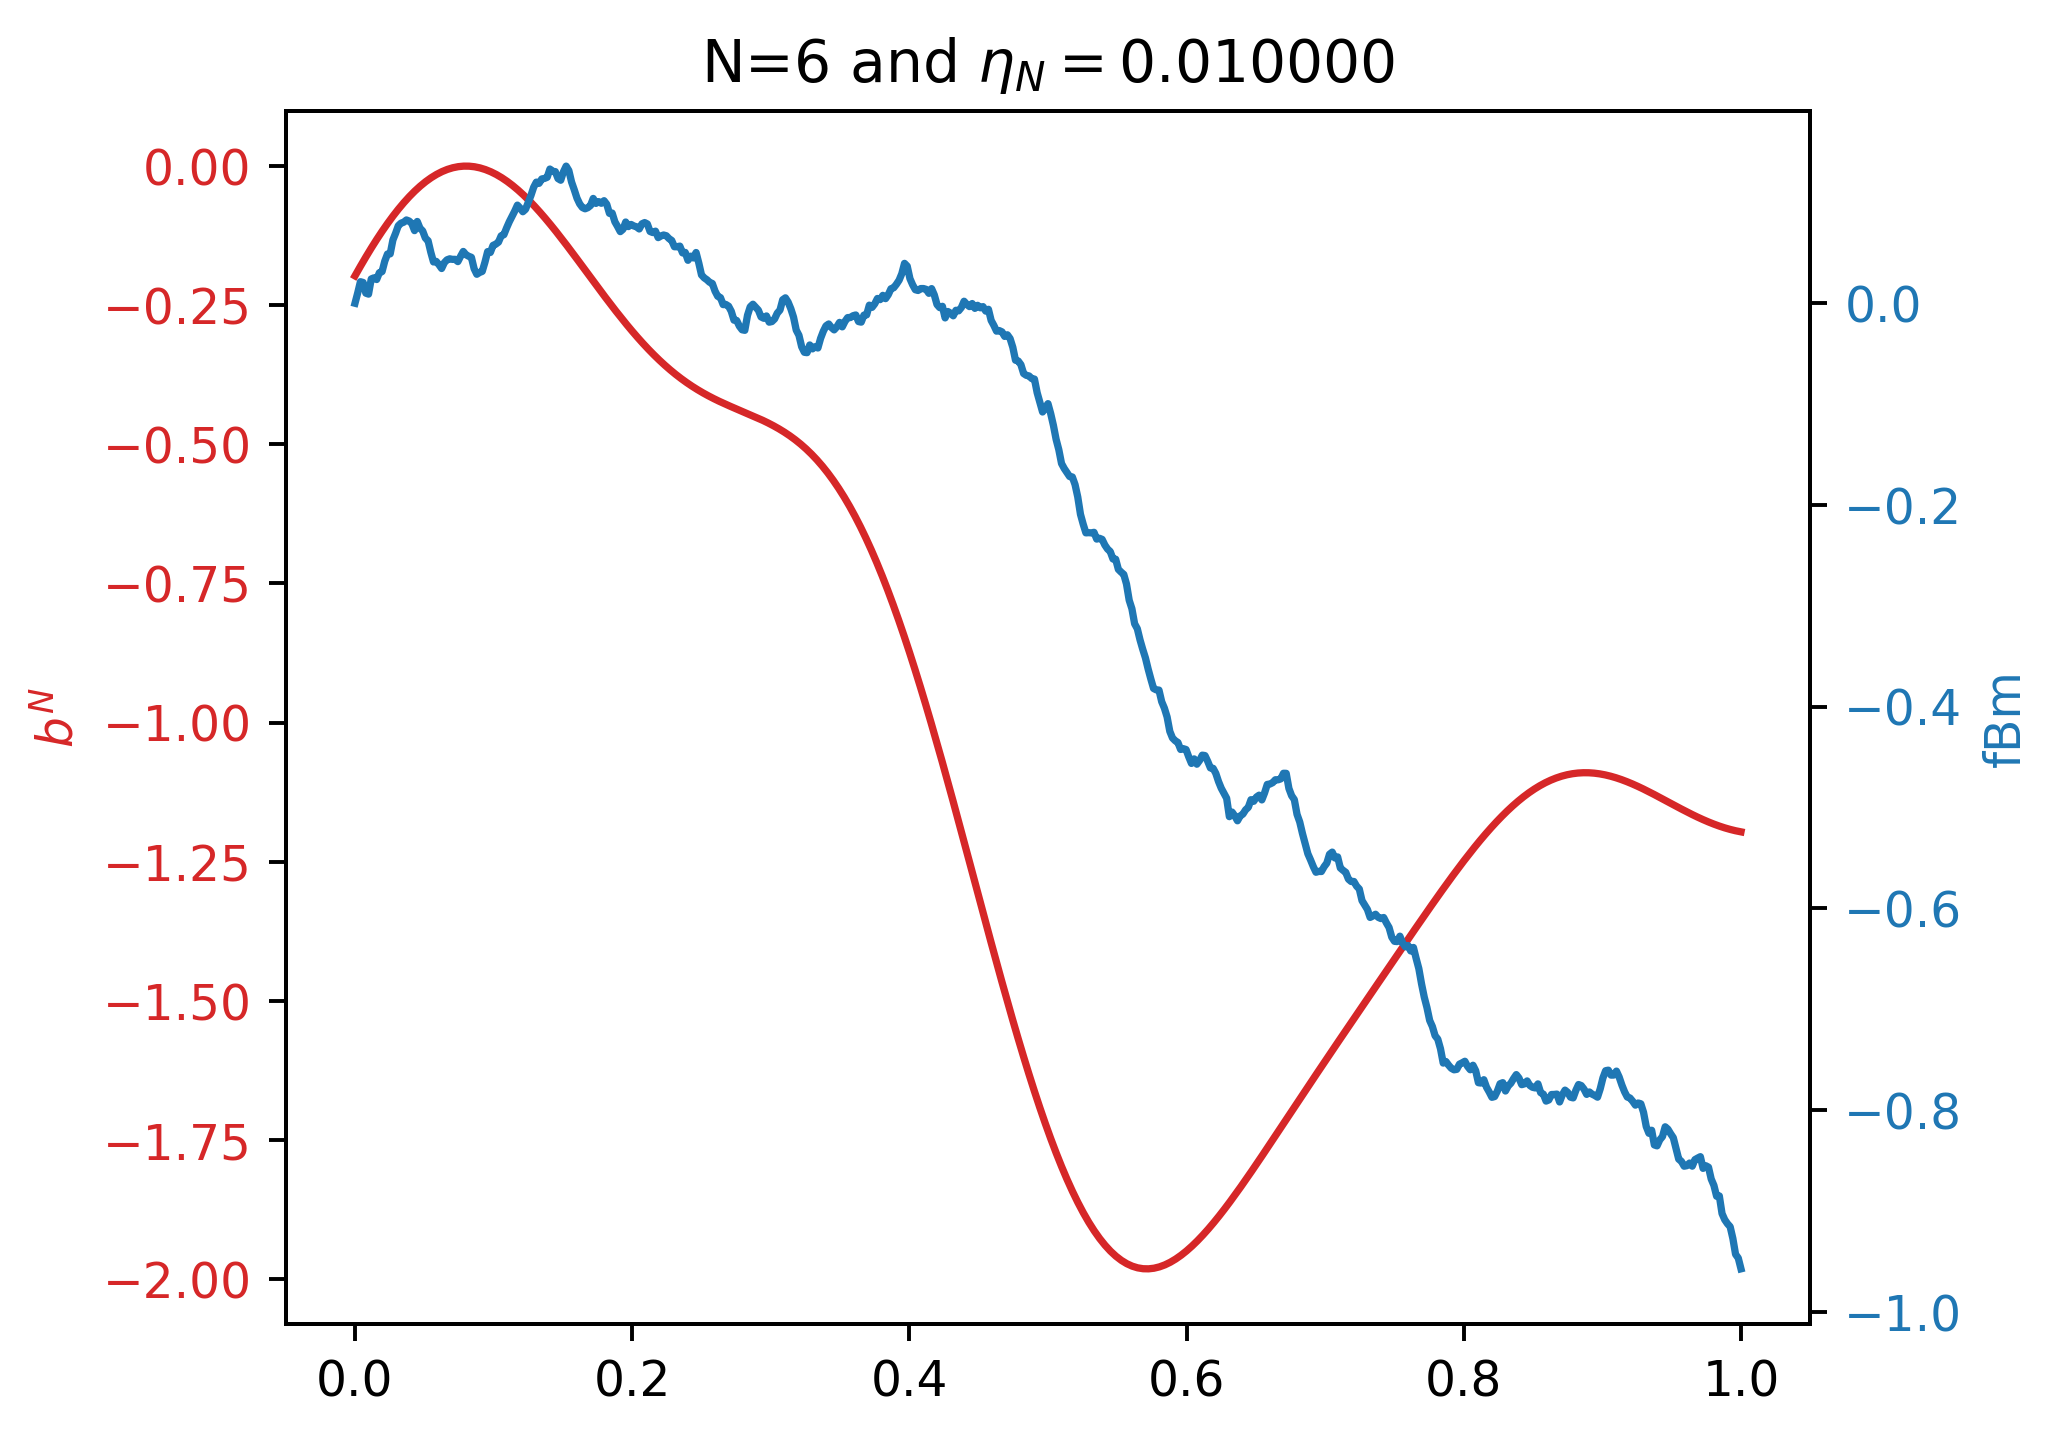
\includegraphics[width=0.49\textwidth]{bn_n6_eta01}
				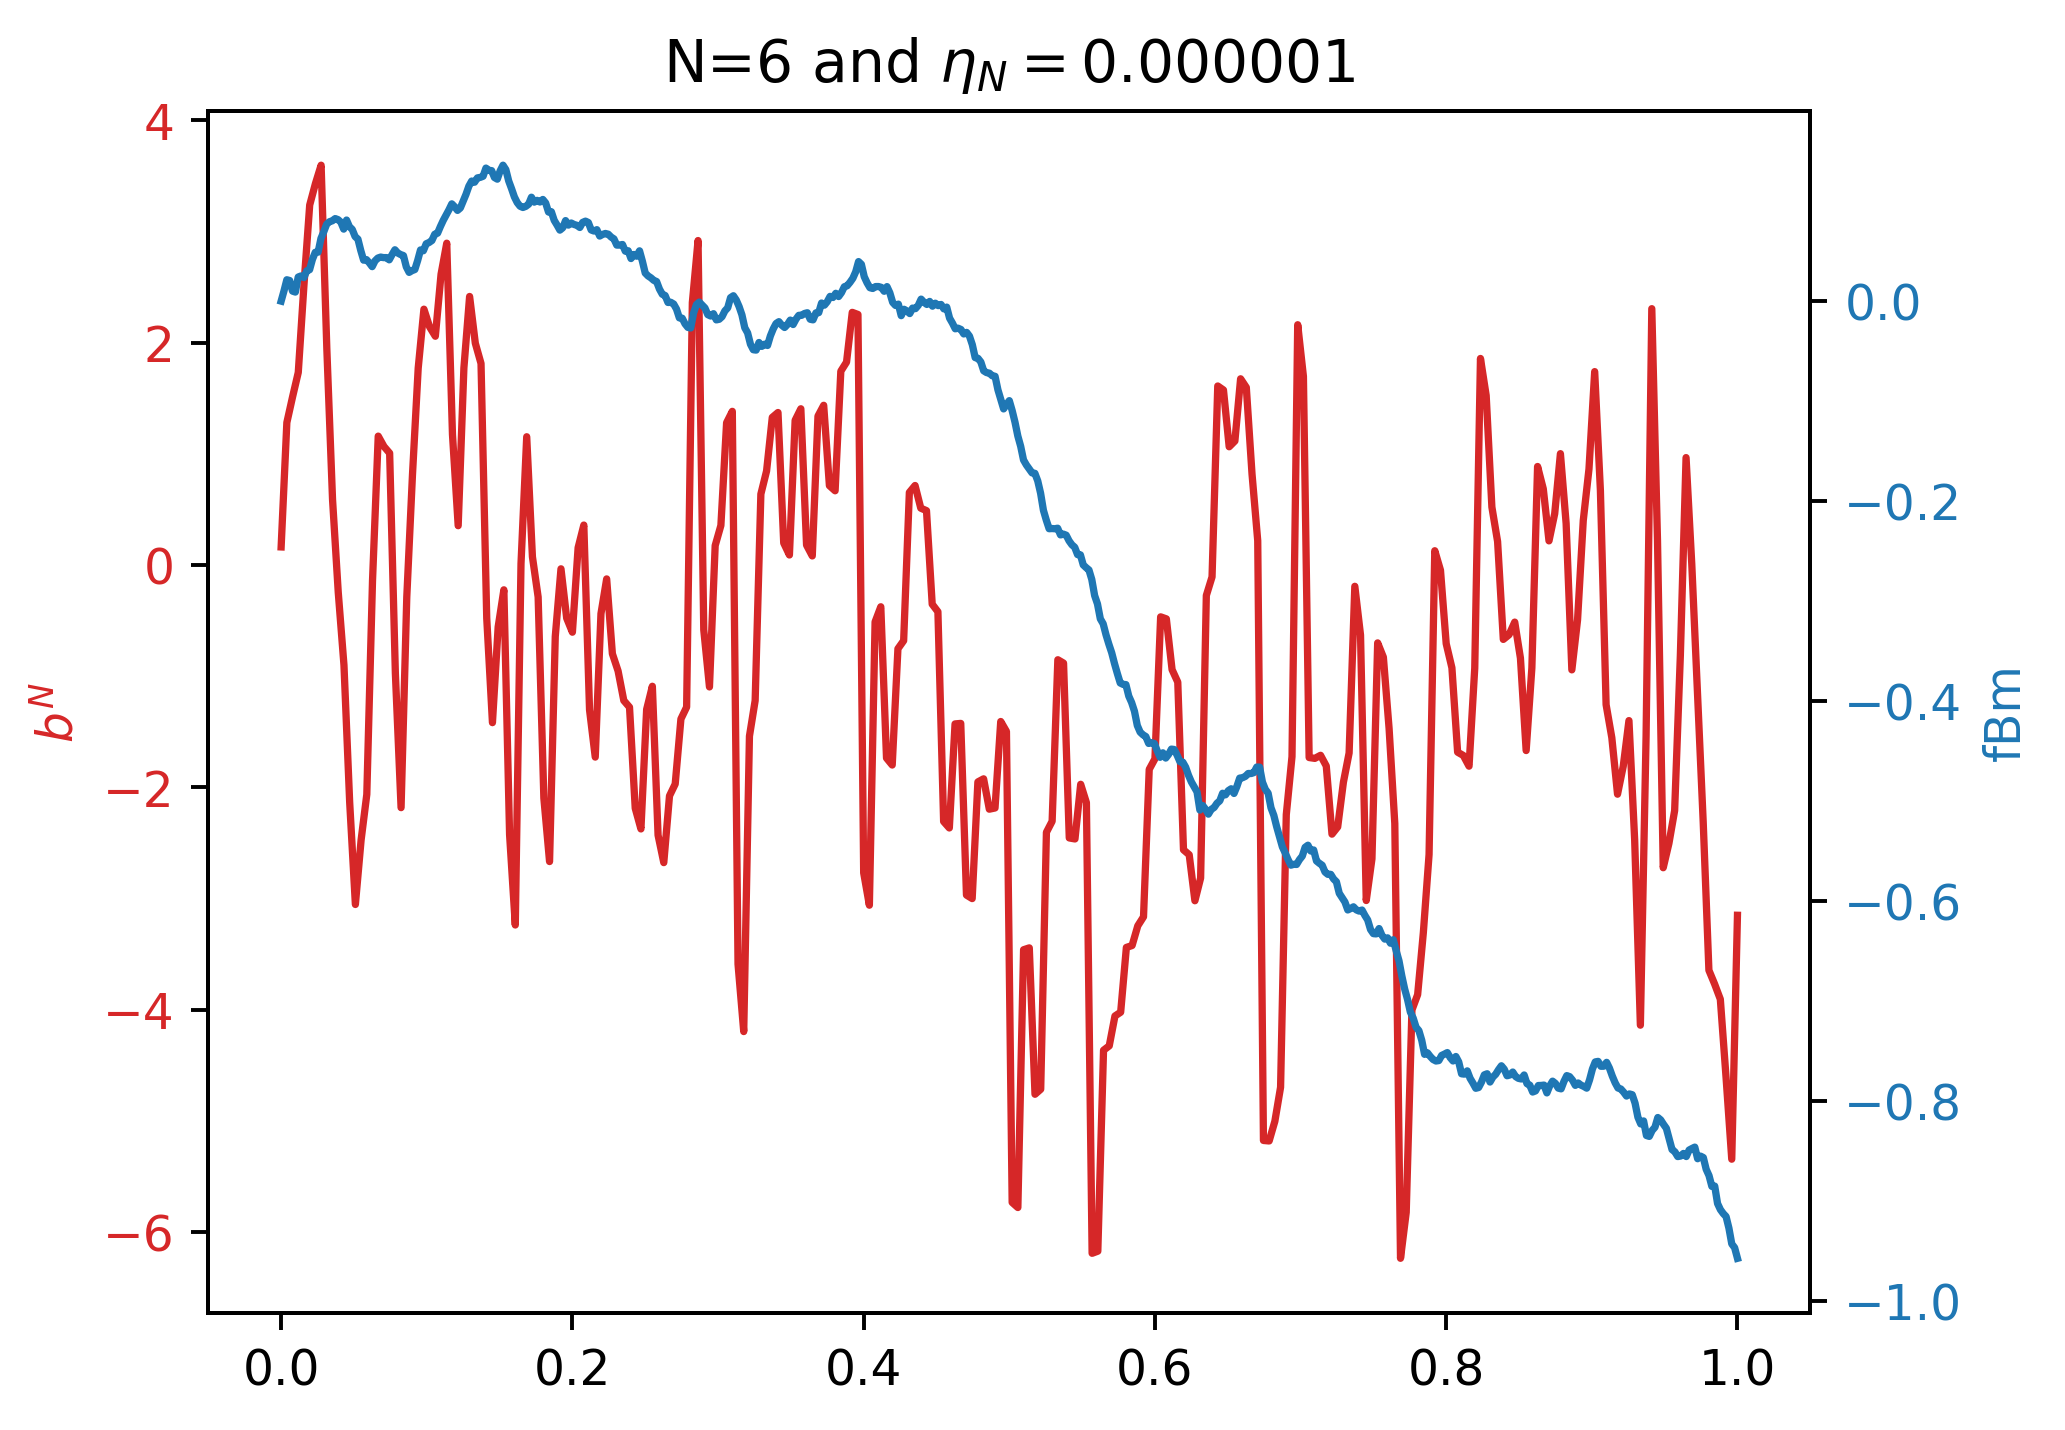
\includegraphics[width=0.49\textwidth]{bn_n6_eta501}
				\caption{Coefficient $P_{\eta_{N}}b^{N}$ for $N=6$ and $\eta=10^{-2}, 10^{-6}$.}
		\end{figure}
\end{frame}

\begin{frame}{Implementation}
		\begin{figure}
				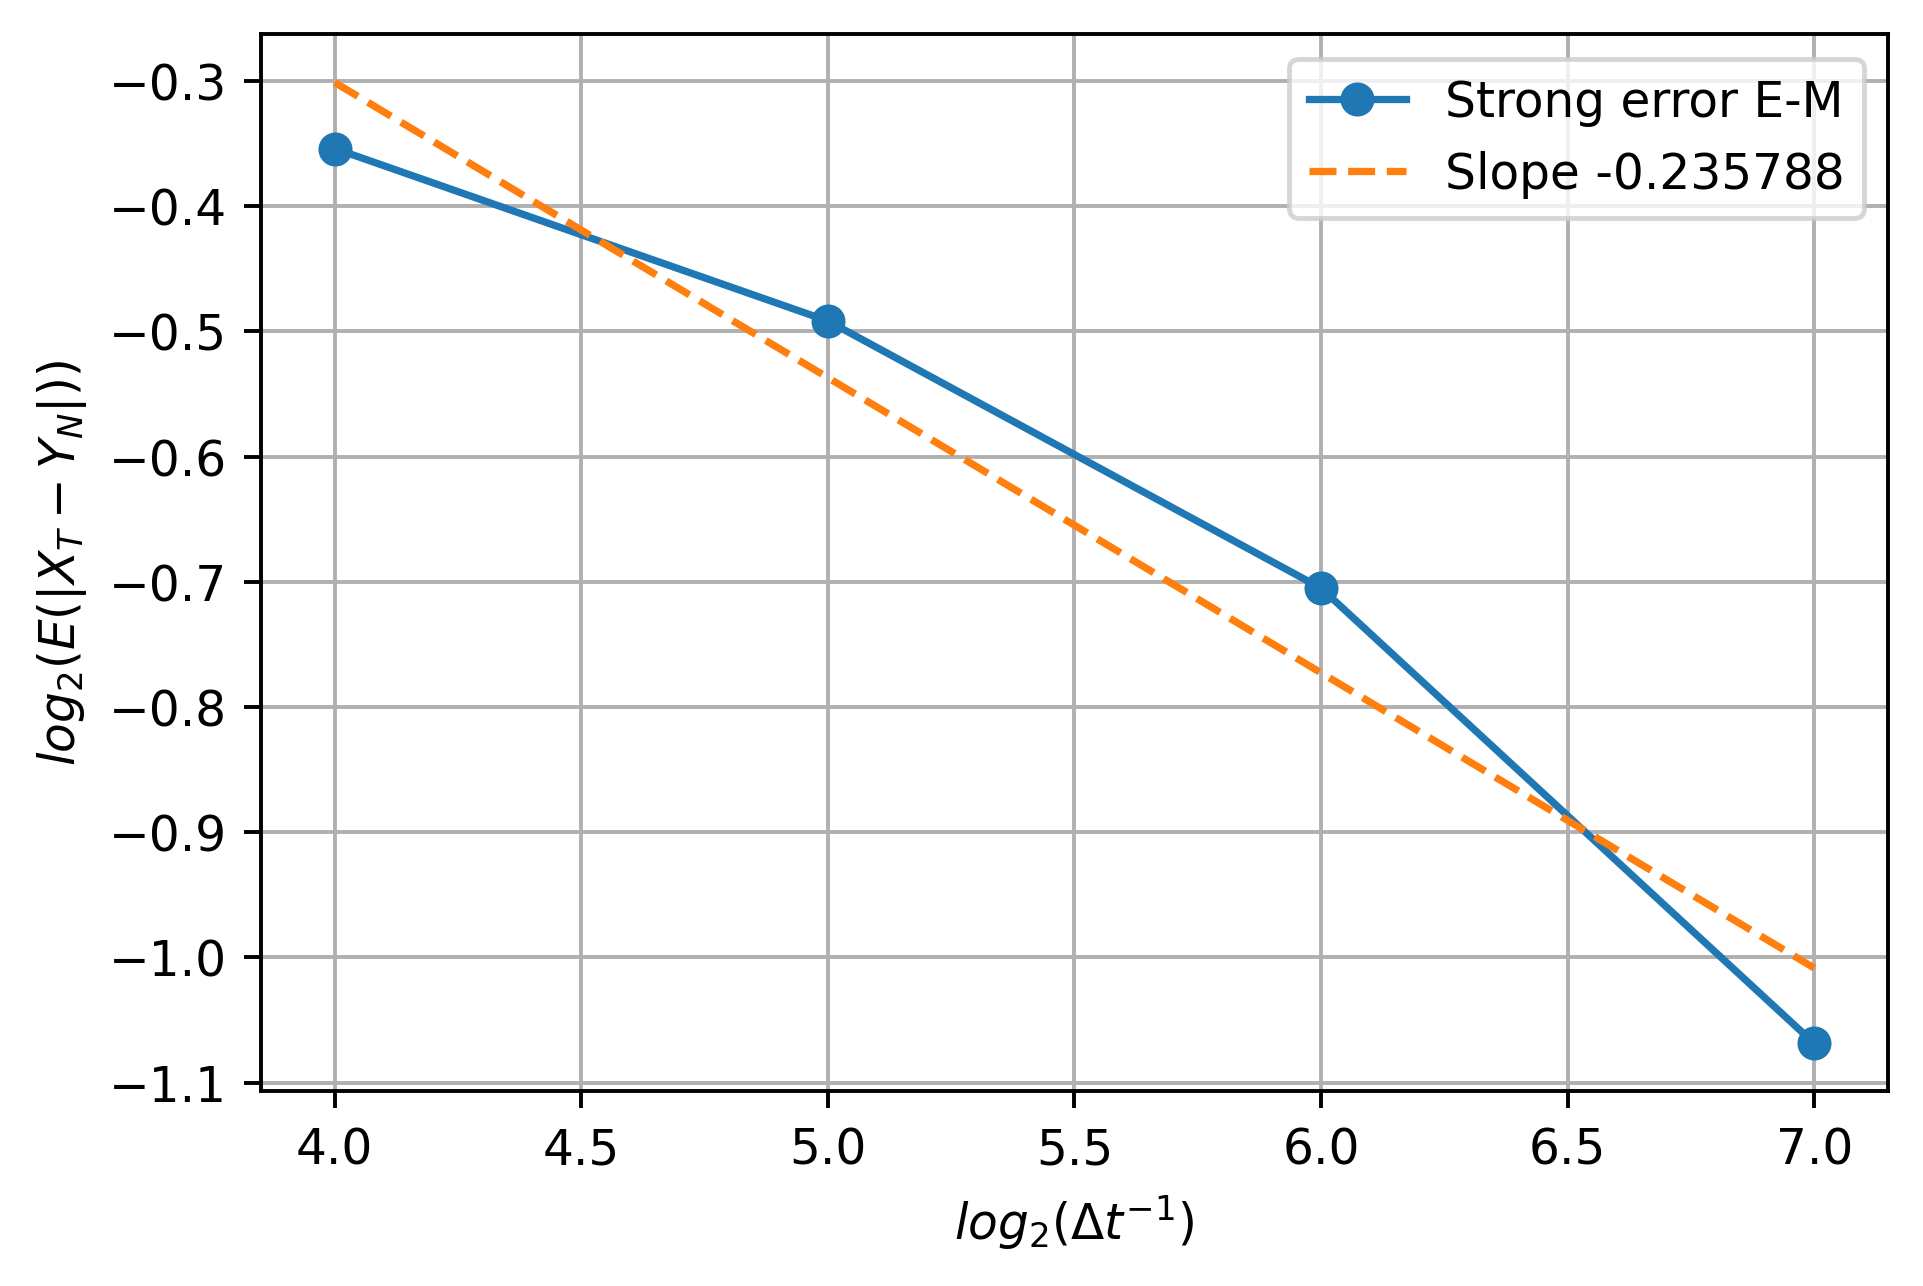
\includegraphics[width=0.7\textwidth]{distributional_2_4_2_7_error}
				\caption{Error of the Euler scheme for the approximation of the distributional coefficient for real solution with $2^9$ time steps and approximations with $2^4$ to $2^7$ time steps, $ b \in H^{-0.05}_{2,q_0} $ and $q_0>4$.}
		\end{figure}
\end{frame}

\begin{frame}[allowframebreaks]{References}
        \printbibliography
\end{frame}

\end{document}
